\setAuthor{Tundmatu autor}
\setRound{lahtine}
\setYear{2006}
\setNumber{G 7}
\setDifficulty{6}
\setTopic{Staatika}

\prob{Kuul}
Kasti tasasel põhjal asub kuul. Kasti põhi asub nurga all horisontaalsuuna suhtes. Kuuli hoiab tasakaalus kasti seina külge kinnitatud niit, mis on paralleelne kasti põhjaga (vt joonist). Kui suure maksimaalse nurga $\varphi$ võrra saab kasti kallutada, et kuul oleks veel tasakaalus? Hõõrdetegur kuuli ja kasti vahel on $\mu$.

\begin{center}
	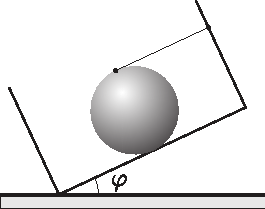
\includegraphics[width=0.5\linewidth]{2006-lahg-07-yl}
\end{center}

\hint
Kuulile mõjub raskusjõud, niidi pinge, toereaktsioon ning hõõrdejõud kuuli ja kasti vahel. Süsteemi lahendamise standardmeetod on rakendada Newtoni II seadust nii $x$- kui ka $y$-telje jaoks ning jõumomentide tasakaalu tingimust. Elu teeb lihtsamaks tähelepanek, et hõõrdejõu ja toereaktsiooni võib kombineerida üheks jõuks, mille nurk kasti vertikaali suhtes on kuni $\arctan\mu$ ning seejärel täheldada, et tasakaalu korral peavad kuulile mõjuvad kolm jõudu lõikuma ühes punktis.

\solu
Kõigepealt uurime kuulile mõjuvate jõudude projektsioone kasti põhjaga risti olevale teljele (vt joonist).

\begin{center}
	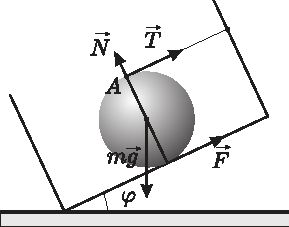
\includegraphics[width=0.5\linewidth]{2006-lahg-07-lah}
\end{center}

Nende projektsioonide summa peab olema võrdne nulliga. Projektsioone sellele teljele omavad vaid raskusjõud $m\vec g$ ja kasti põhja toereaktsioon $\vec N$. Järelikult
$N = mg \cos \varphi$ ja hõõrdejõud
\begin{equation} \label{2006-lahg-07:e1}
F \leq \mu mg \cos\varphi.
\end{equation}
Kuuli tasakaal sõltub selle võrratuse täitumisest.

Nüüd tuleb valida punkt, mille suhtes me hakkame määrama jõumomente. Valime punkti nii, et hõõrdejõu moment selle suhtes oleks nullist erinev, aga niidi tõmbepinge $T$ moment oleks võrdne nulliga (niidi pinge arvutamise vältimiseks). Sellele tingimusele vastab punkt $A$, milles niit kinnitub kuuli külge. Selle punkti suhtes on hõõrdejõu õlg $2r$ (kus $r$ on kuuli raadius), raskusjõu õlg $l = r \sin \varphi$, ning jõudude $N$ ja $T$ õlad võrdsed nulliga. Jõumomentide summa on tasakaalu puhul võrdne nulliga, järelikult
\[
2 r F-m g r \sin \varphi=0 \quad \Rightarrow \quad F=\frac{m g \sin \varphi}{2}.
\]
Arvestades võrratust (\ref{2006-lahg-07:e1}) leiame, et tasakaalu puhul
\[
\mu m g \cos \varphi \geq \frac{m g \sin \varphi}{2} \Rightarrow \tan \varphi=2 \mu,
\]
ehk
\[
\varphi = \arctan (2\mu).
\]
\probend